\documentclass{standalone}

\usepackage{tikz}

\usetikzlibrary{positioning, chains, shapes.geometric, fit, shapes, arrows.meta, calc, backgrounds}

\begin{document}

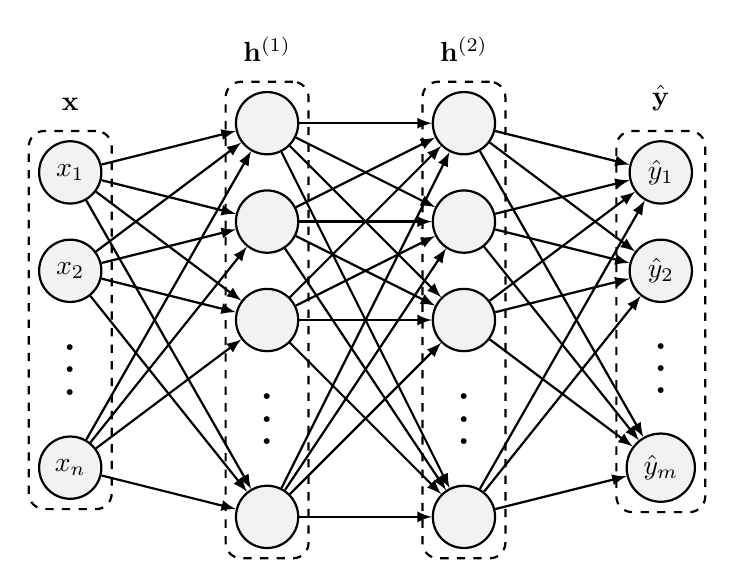
\begin{tikzpicture}[
    >=LaTeX, % Use default LaTeX arrows
    % Styles 
    node/.style={ % Input or output node
        circle,
        minimum width=2.25em,
        draw,
        fill=gray!10,
        thick
    },
    cell/.style={
        rectangle,
        rounded corners=2mm,
        minimum height=2.5em,
        minimum width=2.5em,
        draw,
        thick
    }, 
    arrow/.style={
        -latex,
        thick
    },
    backprop/.style={ % Backpropagation arrows
        arrow,
        dashed,
        gray
    }
]
    	
    % Input
    \foreach \x in {1,...,2}
        \draw node at (0, -\x*1.25 - 0.625) [node] (first_\x) {$x_\x$};
    \draw node at (0, -5*1.25 + 0.625) [node] (first_n) {$x_n$};
    \path (first_2) -- (first_n) node[pos=0.38, scale=2] {\vdots};
    	
    % Hidden 1
    \foreach \x in {1,...,3}
        \node at (2.5, -\x*1.25) [node] (second_\x){};
    \draw node at (2.5, -5*1.25) [node] (second_m) {};
    \path (second_3) -- (second_m) node[pos=0.38, scale=2] {\vdots};

    % Hidden 2
    \foreach \x in {1,...,3}
        \node at (5, -\x*1.25) [node] (third_\x){};
    \draw node at (5, -5*1.25) [node] (third_m) {};
    \path (third_3) -- (third_m) node[pos=0.38, scale=2] {\vdots};
    	
    % Output
    \foreach \x in {1,...,2}
        \node at (7.5, -\x*1.25 - 0.625) [node] (fourth_\x){$\hat{y}_\x$};
    \draw node at (7.5, -5*1.25 + 0.625) [node] (fourth_k) {$\hat{y}_m$};
    \path (fourth_2) -- (fourth_k) node[pos=0.38, scale=2] {\vdots};
    		
    % Input -> Hidden
    \foreach \i in {1,...,2}
        \foreach \j in {1,...,3}
            \draw [arrow] (first_\i) to (second_\j);
    \foreach \i in {1,...,2}
        \draw [arrow] (first_\i) to (second_m);
    \foreach \i in {1,...,3}
        \draw [arrow] (first_n) to (second_\i);
    \draw [arrow] (first_n) to (second_m);

    % Hidden -> Hidden
    \foreach \i in {1,...,3}
        \foreach \j in {1,...,3}
            \draw [arrow] (second_\i) to (third_\j);
    \foreach \i in {1,...,3}
        \draw [arrow] (second_\i) to (third_m);
    \foreach \i in {1,...,3}
        \draw [arrow] (second_m) to (third_\i);
    \draw [arrow] (second_m) to (third_m);
    	
    % Hidden -> Output
    \foreach \i in {1,...,3}
        \foreach \j in {1,...,2}
            \draw [arrow] (third_\i) to (fourth_\j);
    \foreach \i in {1,...,3}
        \draw [arrow] (third_\i) to (fourth_k);
    \foreach \i in {1,...,2}
        \draw [arrow] (third_m) to (fourth_\i);
    \draw [arrow] (third_m) to (fourth_k);
    	
    % Layer Labels
    \node[above=0.25cm of first_1] (xlabel) {$\mathbf{x}$};
    \node[above=0.25cm of second_1] (h1label) {$\mathbf{h}^{(1)}$};
    \node[above=0.25cm of third_1] (h2label) {$\mathbf{h}^{(2)}$};
    \node[above=0.25cm of fourth_1] (ylabel) {$\hat{\mathbf{y}}$};

    \node[cell, dashed, fit=(first_1) (first_n)] (xbox) {};
    \node[cell, dashed, fit=(second_1) (second_m)] (xbox) {};
    \node[cell, dashed, fit=(third_1) (third_m)] (xbox) {};
    \node[cell, dashed, fit=(fourth_1) (fourth_k)] (xbox) {};
\end{tikzpicture}

\end{document}